% Compiler XeLaTeX
\documentclass{article}
\usepackage{geometry}
\geometry{a4paper,scale=0.8}
\usepackage[utf8]{inputenc}
\usepackage[backend = biber, sorting = none]{biblatex}
\addbibresource{references.bib}
\usepackage{url}
\usepackage{graphicx}
\graphicspath{ {image/} }
\usepackage{booktabs}
\usepackage{caption}
\usepackage{amsmath}
\usepackage{enumitem}
\usepackage[UTF8]{ctex}
\usepackage[
	colorlinks,
	linkcolor = black,     
	urlcolor = black,
	citecolor = black
]{hyperref}

\title{Report}
\date{}

\begin{document}

\maketitle

Codes are available at \url{https://github.com/Tsianmy/Stereo}.

%%%%%%%%%%%%%%%%%%%%%%%%%%
% Camera Basics
%%%%%%%%%%%%%%%%%%%%%%%%%%
\section*{Camera Basics}
\begin{enumerate}

%%%%%%%%%%%%%%%%%%%%%%%%%%
% 1
%%%%%%%%%%%%%%%%%%%%%%%%%%
\item From Wikipedia, we learn that \textbf{intrinsics} of a camera can be represented by a matrix $K$ \cite{ref1}, 

$$
K =
\begin{bmatrix}
f_x & s & c_x & 0 \\
0 & f_y & c_y & 0 \\
0 & 0 & 1 & 0
\end{bmatrix},
$$

$f_x = f \cdot m_x$ and $f_y = f \cdot m_y$ , where $m_x$ and $m_y$ are the scale factors relating the $x$ and the $y$ axis, $f$ is the focal length, $c_x$ and $c_y$ represent the center point of the image, $s$ is the skew coefficient along the $x$-axis and the $y$-axis, and is often $0$.

In some books and articles \cite{ref2}\cite{ref3}, $K$ is represented as $\begin{bmatrix} f_x & 0 & c_x \\ 0 & f_y & c_y \\ 0 & 0 & 1 \end{bmatrix}$. Maybe it's because there's a transformation from homogeneous coordinates to nonhomogeneous coordinates. These two matrices are essentially equivalent.

$R, t$ are the \textbf{extrinsics} which denote the coordinate system transformations from 3D world coordinate to 3D camera coordinate \cite{ref1}. The isometry matrix is $\begin{bmatrix} R & t \\ \boldsymbol 0^\mathrm T & 1 \end{bmatrix}$.

Finally, the \textbf{camera matrix} is $M = K \begin{bmatrix} R \quad t \end{bmatrix}$.

%%%%%%%%%%%%%%%%%%%%%%%%%%
% 2
%%%%%%%%%%%%%%%%%%%%%%%%%%
\item Suppose the coordinate in the image plane is $\boldsymbol X' = \begin{bmatrix} u \\ v \\ 1 \end{bmatrix}$, then

$$
\boldsymbol X' = \begin{bmatrix} u \\ v \\ 1 \end{bmatrix} = \frac 1Z K(R\boldsymbol X + t) = \frac 1Z \begin{bmatrix} f_x & 0 & c_x \\ 0 & f_y & c_y \\ 0 & 0 & 1 \end{bmatrix} \begin{bmatrix} R \quad t \end{bmatrix} \begin{bmatrix} X_1 \\ X_2 \\ X_3 \\ 1 \end{bmatrix}.
$$

%%%%%%%%%%%%%%%%%%%%%%%%%%
% 3
%%%%%%%%%%%%%%%%%%%%%%%%%%
\item A 2D image point corresponds to a line in the 3D camera coordinate because its depth is unknown. 

Let the point be $\boldsymbol P_{uv} = \begin{bmatrix} u \\ v \end{bmatrix}$ in the 2D coordinate and $\boldsymbol P_c = \begin{bmatrix} X \\ Y \\ Z \end{bmatrix}$ in the camera coordinate. We have 
the equation

$$
\begin{bmatrix} u \\ v \\ 1 \end{bmatrix} = \frac 1Z \begin{bmatrix} f_x & 0 & c_x \\ 0 & f_y & c_y \\ 0 & 0 & 1 \end{bmatrix} \begin{bmatrix} X \\ Y \\ Z \end{bmatrix},
$$

then,

$$
\boldsymbol P_c = \begin{bmatrix} X \\ Y \\ Z \end{bmatrix} = ZK^{-1}\boldsymbol P_c = Z \begin{bmatrix} f_x^{-1} & 0 & -f_x^{-1}c_x \\ 0 & f_y^{-1} & -f_y^{-1}c_y \\ 0 & 0 & 1 \end{bmatrix} \begin{bmatrix} u \\ v \\ 1 \end{bmatrix}.
$$

As we lack depth information of the 2D image point, value $Z$ is unknown. Let $Z = \lambda$, we have

$$\begin{cases}
X = \lambda (\frac u{f_x} - \frac {c_x}{f_x}) \\
Y = \lambda(\frac v{f_y} - \frac {c_y}{f_y}) \\
Z = \lambda
\end{cases}.$$

And it is a line in the 3D camera coordinate.

%%%%%%%%%%%%%%%%%%%%%%%%%%
% 4
%%%%%%%%%%%%%%%%%%%%%%%%%%
\item \textbf{Distortion} is a deviation from rectilinear projection; a projection in which straight lines in a scene remain straight in an image; It is a form of optical aberration\cite{ref4}. According to the OpenCV documentation, there are two common kinds of distortion: radial distortion and tangential distortion\cite{ref5}.

In the radial distortion model, the actual projected point is related to the ideal point by a radial displacement,
$$
\boldsymbol X_d = \begin{bmatrix} x_d \\ y_d \end{bmatrix} = L(r) \begin{bmatrix} x_u \\ y_u \end{bmatrix} = L(r) \boldsymbol X_u ,
$$
where  $\boldsymbol X_u$ is the ideal image position, $\boldsymbol X_d$ is the distorted position, $r$ is the radial distance $\sqrt{x_u^2 + y_u^2}$ and  $L(r)$ is a distortion factor; An approximation to an arbitrary function $L(r)$ can be given by a Taylor expansion $L(r) = 1 + k_1r + k_2r^2 + k_3r^3 + ...$ \cite{ref6}.

Many articles point out that tangential distortion is minimally characterized by two additional parameters: $p_1$ and $p_2$ \cite{ref5}\cite{ref7}, but the authors didn't explain why the equation could be used to approximate. For tangential distortion, the work by D.C.Brown recasts the extended expressions for Conrady's model into the form \cite{ref8},
$$\Delta_x = [P_1(r^2 + 2x^2) + 2P_2xy][1 + P_3r^2 + P4r^2 + ...]$$
$$\Delta_y = [2P_1xy + P_2(r^2 + 2y^2)][1 + P_3r^2 + P4r^2 + ...].$$

Now the simplified expression used in the distortion model is
$$\begin{aligned}
x_{distorted} &= x + 2p_1xy + p_2(r^2+2x^2)\\
y_{distorted} &= y + p_1(r^2+ 2y^2)+ 2p_2xy
\end{aligned}$$

With two kinds of distortion, the distorted position is
$$\begin{cases}
x_{distorted} = x(1 + k_1r^2 + k_2r^4 + k_3r^6) + 2p_1xy + p_2(r^2+2x^2) \\
y_{distorted} = y(1 + k_1r^2 + k_2r^4 + k_3r^6) + p_1(r^2+ 2y^2)+ 2p_2xy
\end{cases}.$$

Given a 2D image point $(u, v)$, the position in the camera coordinate is
$$\begin{cases}
x = \frac{u - c_x}{f_x} \\
y = \frac{v - c_y}{f_y}
\end{cases}.$$

So the distorted position is
$$\begin{cases}
x_{distorted} = x(1 + k_1r^2 + k_2r^4) + 2p_1xy + p_2(r^2+2x^2) \\
y_{distorted} = y(1 + k_1r^2 + k_2r^4) + p_1(r^2+ 2y^2)+ 2p_2xy
\end{cases}.$$

Lastly, the correct position is
$$\begin{cases}
u_{undistorted} = f_xx_{distorted} + c_x \\
v_{undistorted} = f_yy_{distorted} + c_y
\end{cases}.$$

%%%%%%%%%%%%%%%%%%%%%%%%%%
% 5
%%%%%%%%%%%%%%%%%%%%%%%%%%
\item \textbf{Camera calibration} involves finding the intrinsics and extrinsics of a camera with distortion if it is considered.

Wikipedia explains that camera calibration is the process of estimating the parameters of a camera model approximating the camera that produced a given photograph or video, many people restrict the term camera calibration for the estimation of internal or intrinsic parameters only \cite{ref1}.

Similarly, it is said in the book "Learning OpenCV 3" that the process of camera calibration gives us both a model of the camera’s geometry and a distortion model of the lens which define the intrinsic parameters of the camera \cite{ref9}.

Many algorithms have been developed to calculate the parameters.

%%%%%%%%%%%%%%%%%%%%%%%%%%
% 6
%%%%%%%%%%%%%%%%%%%%%%%%%%
\item The OpenCV calibration document lists the APIs and the tutorials show the steps of calibration as well as the OpenCV book \cite{ref9}\cite{ref10}.
\begin{itemize}
  \item First of all, read the image and use function \verb|cv::findChessboardCorners()| to locate the corners of the chessboard.
  \item Call \verb|cv::cornerSubPix()| to locate better.
  \item Call \verb|cv::calibrateCamera()| to get intrinsic matrix, the distortion coefficients, and the extrinsics.
	\item Fit a homography matrix for all the images.
\end{itemize}

The result indicates that chessboard corners can be well-detected (Figure 6-1), but it's hard to tell whether the matrix is fitted well (see the parameters in Table 6-1).
\begin{figure}[h]
	\centering
	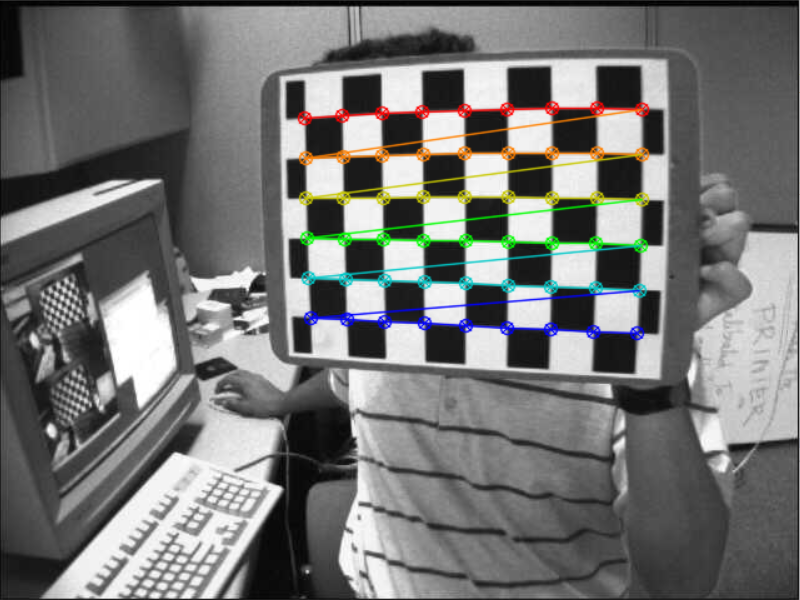
\includegraphics[width=0.4\textwidth]{6-1}
	\caption*{Figure 6-1. The corners of chessboard}
\end{figure}

\begin{table}[h]
	\caption*{Table 6-1. Intrinsics and distortion coefficients}
	\centering
	\begin{tabular}{ccc|cc}
		\toprule[2pt]
		\multicolumn{3}{c|}{intrinsics} & \multicolumn{2}{c}{distortion coefficients($k_1, k_2, p_1, p_2, k_3$)} \\ \hline
		102.67     & 0         & 320    & -0.029448            & 2.691e-05            \\
		0          & 385.38    & 240    & 0                    & 0                    \\
		0          & 0         & 1      & 1.019e-07            &                      \\
		\bottomrule[2pt]
	\end{tabular}
\end{table}

%%%%%%%%%%%%%%%%%%%%%%%%%%
% 7
%%%%%%%%%%%%%%%%%%%%%%%%%%
\item For undistortion, we use function \verb|cv::initUndistortRectifyMap()| to compute the undistortion maps and function \verb|cv::remap()| to apply them to the images.

However, the result are not satisfactory (see Figure 7-1). The images are from the examples of OpenCV and there are the parameters of a good fit. After comparing the parameters, we find that there is a certain amount of error between the parameters. We try to use the parameters of example to undistort the image and the result is in Figure 7-2. It indicates that the undistortion was perfect. 

\begin{figure}[h]
\centering
\begin{minipage}[]{0.45\textwidth}
\centering
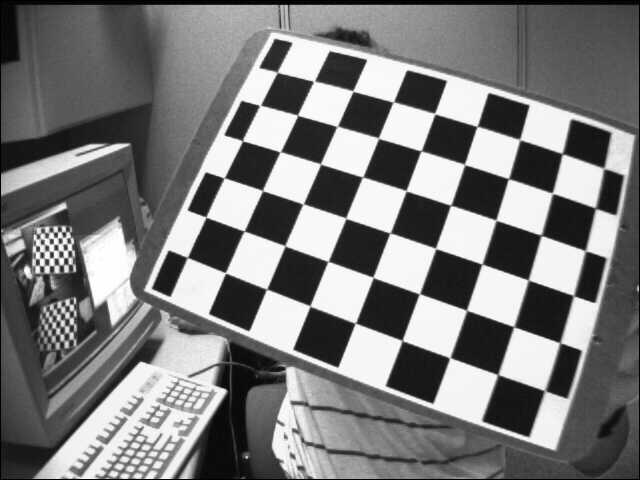
\includegraphics[width=6cm]{7-1l}
\end{minipage}
\begin{minipage}[]{0.45\textwidth}
\centering
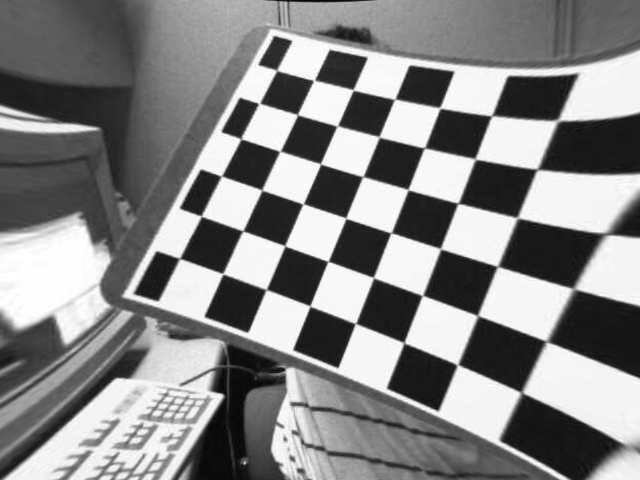
\includegraphics[width=6cm]{7-1r}
\end{minipage}
\caption*{Figure 7-1. Original image(left) and undistorted image(right)}
\end{figure}

We attempt to use fewer images to input but it doesn't work. When comparing the codes with example codes of OpenCV, we discover that the vector which contains the coordinate values of the points on the calibration pattern for a particular image requires an order of XYZ-dimension. After we correct the order, the corresponding image is almost the same as Figure 7-2.

And the latest parameters are in Table 7-1. The average projection error is $\textbf{0.39282}$.

\begin{figure}[h]
	\centering
	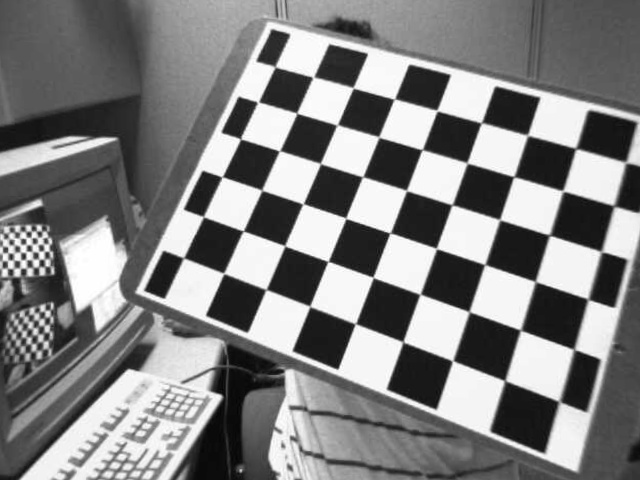
\includegraphics[width=0.4\textwidth]{7-2}
	\caption*{Figure 7-2. Undistortion with parameters of sample}
\end{figure}

\begin{table}[h]
	\caption*{Table 7-1. Intrinsics and distortion coefficients after correction}
	\centering
	\begin{tabular}{ccc|cc}
		\toprule[2pt]
		\multicolumn{3}{c|}{intrinsics} & \multicolumn{2}{c}{distortion coefficients($k_1, k_2, p_1, p_2, k_3$)} \\ \hline
		535.89     & 0         & 342.29    & -0.2662           & -3.968e-02           \\
		0          & 535.84    & 235.52    & 1.794e-03         & -2.988e-04           \\
		0          & 0         & 1     		 & 2.401e-01         &                      \\
		\bottomrule[2pt]
	\end{tabular}
\end{table}

%%%%%%%%%%%%%%%%%%%%%%%%%%
% 8
%%%%%%%%%%%%%%%%%%%%%%%%%%
\item Zhang's method can be summarized in mainly 6 steps \cite{ref11}.
\begin{itemize}
	\item Capture images from different perspective and detect corners.
	\item Solve $\widetilde{m} = H \widetilde{M}$ for each image, where $\widetilde{m}$ is a 2D point, $\widetilde{M}$ is a 3D point and homography $H = A[r1 \; r2\; t]$.
	\item Solve equation $vb = 0$ to get $B$ and get intrinsics by decomposing $B$.
	\item Calculate extrinsic matrix $[R \; t]$.
	\item Solve $Dk = d$ to get distortion parameters.
	\item Optimize the parameters by Levenberg-Marquardt Algorithm.
\end{itemize}

The codes are referenced to Eating Lee's blog \cite{ref12} and the parameters are in Table 8-1.

\begin{table}[h]
	\caption*{Table 8-1. Intrinsics and distortion coefficients}
	\centering
	\begin{tabular}{ccc|cc}
		\toprule[2pt]
		\multicolumn{3}{c|}{intrinsics} & \multicolumn{2}{c}{distortion coefficients($k_1, k_2$)} \\ \hline
		536.01     & 2.337     & 352.61    & 0.11478           & -0.10458         	  \\
		0          & 537.19    & 236.12    & 					         & 						          \\
		0          & 0         & 1     		 & 					         &                      \\
		\bottomrule[2pt]
	\end{tabular}
\end{table}

The average projection error is $\textbf{3.05258}$ and it's less precise than the projection (error $\textbf{0.39282}$) in Problem 6.

\end{enumerate}

%%%%%%%%%%%%%%
As the derivation of Problem 3, it's hard to estimate the depth of the pixels with a single camera and a single image. But there exist some methods to estimate depth such as estimating objects with handicraft. The better way is using two cameras to estimate depth.
%%%%%%%%%%%%%%

%%%%%%%%%%%%%%%%%%%%%%%%%%
% Binocular Basics
%%%%%%%%%%%%%%%%%%%%%%%%%%
\section*{Binocular Basics}

\begin{enumerate}[resume]

%%%%%%%%%%%%%%%%%%%%%%%%%%
% 9
%%%%%%%%%%%%%%%%%%%%%%%%%%
\item Because the 3D world coordinate is set as the 3D camera coordinate of the left camera, the projection in left plane is
$$
\boldsymbol{X'_l} = \frac{1}{X_3} M_l \boldsymbol{X} = \frac{1}{X_3} \begin{bmatrix} \frac{X_1 - c_x}{f_x} \\ \frac{X_2 - c_y}{f_y} \\ X_3 \end{bmatrix} ,
$$

The projection in right plane is
$$
\boldsymbol{X'_r} = \frac{1}{X_3} M_r [R \quad t] \boldsymbol{X} = \frac{1}{X_3} M_r [R \quad t] \begin{bmatrix} X_1 \\ X_2 \\ X_3 \\ 1 \end{bmatrix} .
$$

%%%%%%%%%%%%%%%%%%%%%%%%%%
% 10
%%%%%%%%%%%%%%%%%%%%%%%%%%
\item Figure 10-1 shows the projection of points and the derivation is referenced to an article \cite{ref13}. Let $x_l = \begin{bmatrix} u & v \end{bmatrix}^\mathrm T$, then the 3D point in world coordinate is
$$
\boldsymbol X = s_lM_l^{-1}x_l .
$$

Considering the projection on the right plane, we have
$$
s_rx_r = M_r(R(s_lM_l^{-1}x_l) + t) .
$$

Let $p_r = s_rM_r^{-1}x_r, p_l = s_lM_l^{-1}x_l$,
$$
p_r = Rp_l + t.
$$

Then the left part and the right part of equation both make a cross-product with $t$,
$$
t \times p_r = t \times Rp_l + t \times t .
$$

Consider that $t \times t = 0$,
$$
t \times p_r = t \times Rp_l .
$$

At last, multiply $p_r^\mathrm T$,
$$
p_r^\mathrm T t \times p_r = p_r^\mathrm T t \times Rp_l .
$$

The result of $t \times p_r$ is a vector perpendicular to $p_r$, thus
$$
p_r^\mathrm T t \times Rp_l = x_r^\mathrm T M_r^{-\mathrm T} t \times R M_l^{-1}x_l= 0 .
$$

The equation means $x_r$ lies on the line $l = M_r^{-\mathrm T} t \times R M_l^{-1}x_l$.

\begin{figure}[h]
	\centering
	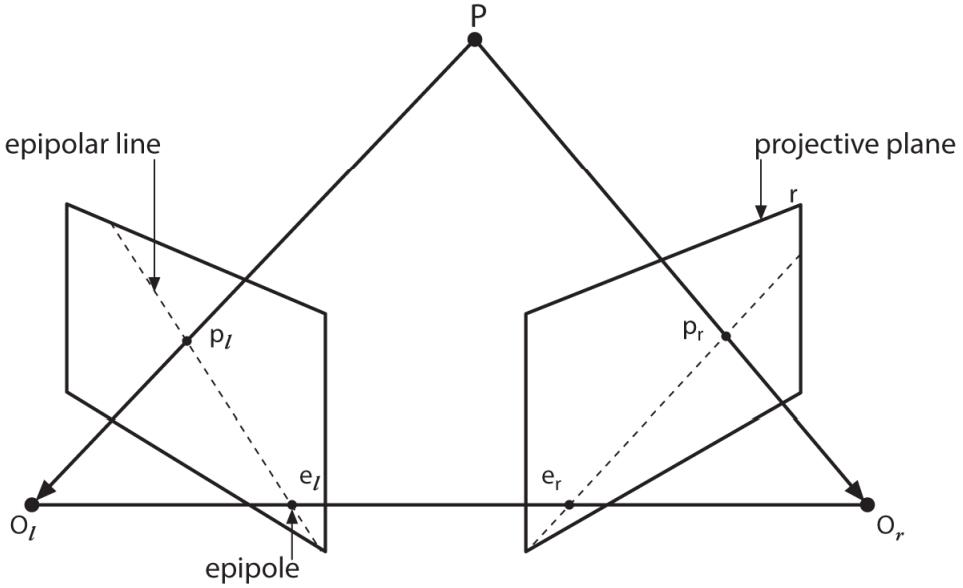
\includegraphics[width=0.45\textwidth]{10-1}
	\caption*{Figure 10-1. Geometry of stereo imaging.}
\end{figure}

%%%%%%%%%%%%%%%%%%%%%%%%%%
% 11
%%%%%%%%%%%%%%%%%%%%%%%%%%
\item Similar to Problem 10, if we swap $x_l$ and $x_r$ and consider $M_r^{-\mathrm T} t \times R M_l^{-1}$ as $F$ , we get $x_l^\mathrm T F x_r = 0$. The book \emph{Learning OpenCV 3} derives from another perspective \cite{ref9}.

Let $p_l = M_l^{-1}x_l, p_r = M_r^{-1}x_r$. The three points are in the same plane, so
$$
(p_l - t)^\mathrm T (t \times p_l) = 0 .
$$

Rewrite $p_r = R(p_l - t)$ as $p_l - t = R^{-1}p_r$ and use $R^{-1} = R^\mathrm T$,
$$
(R^\mathrm T \cdot p_r)^\mathrm T (t \times p_l) = 0 .
$$

Define a skew-symmetric matrix $S$ and rewrite the cross-product,
$$
t \times p_l = S \cdot p_l \Rightarrow S = \begin{bmatrix} 0 & -T_x & T_y \\ T_z & 0 & -T_x \\ -T_y & T_x & 0 \end{bmatrix}.
$$

Hence,
$$
p_r^\mathrm T \cdot R \cdot S \cdot p_l = x_r^\mathrm T M_r^{-\mathrm T} R  S M_l^{-1} x_l = x_r^\mathrm T F x_l = 0.
$$

%%%%%%%%%%%%%%%%%%%%%%%%%%
% 12
%%%%%%%%%%%%%%%%%%%%%%%%%%
\item From moverzp's blog, the parameters to be calibrated are intrinsic matrix, extrinsic matrix, fundamental matrix and distortion coefficients \cite{ref14}. So we follow these steps:
\begin{itemize}
	\item Calculate intrinsics, extrinsics and distortion coefficients of two cameras through methods in above problems.
	\item Calculate the transform $(R | t)$ between the left and the right cameras which is determined by 
	$$
		\begin{cases}
		R = R_rR_l^\mathrm T \\
		T = T_r - RT_l^\mathrm T
		\end{cases}.
	$$
	\item Calculate essential matrix and fundamental matrix.
\end{itemize}

The first encountered issue was that the corners in some images which produced by the right camera couldn't be detected. After referring to OpenCV documentation, we added a flag argument to the function and it worked. Before detection, the function normalizes the image gamma with equalizeHist.

The second issue was how to get the transform $(R | t)$. Each pair of images could generate left and right extrinsic matrices which determined one transform.
\end{enumerate}

\printbibliography[
heading=bibintoc,
title = {References}
]
\end{document}
